\begin{figure}
    \centering
    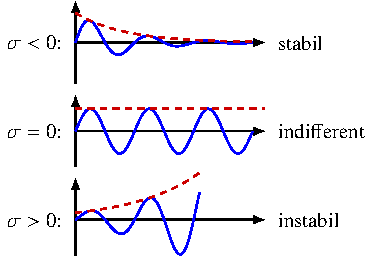
\includegraphics{papers/aircraft/images/eigenwerte.pdf}
    \caption{Die drei möglichen Verläufe von $e^{\lambda t}$ in
    Abhängigkeit vom Realteil $\sigma$ des Eigenwerts.
    Die gestrichelte Hüllkurve $e^{\sigma t}$ ist die Dämpfung, die
    Schwingung darin hat die Frequenz $\omega$.
    Nur für $\sigma < 0$ kehrt die Bewegung in die Ruhelage zurück.
    \label{aircraft:fig:eigenwerte}}
\end{figure}